\chapter{基本動作}\label{basic}

\section{Ruby}\label{ruby}
本研究で学習者が習得するプログラミング言語を決定する.
Rubyとはプログラミング言語の一種であり,少ない記述量で期待する動作を実現できる.
また,西谷研究室で使用を勧めている言語である.
本研究では西谷研究室の早期学習を目的の一つとしているので,本研究で用いる言語はRubyとする.

\section{ユーザーインターフェース}\label{ui}
本研究で開発するアプリケーションで用いる操作方法と動作環境を決定するために,CUI\cite{cui}とGUI\cite{gui}の比較を行う.
CUIとはコンピュータの操作を文字のみで行う方法であり,一方でGUIとはコンピュータの操作をマウスを用いて行う方法である.しかし,GUIでの操作には限界がある.それについて以下に引用を記す.
\begin{quotation}
  GUIでしか作業を行わないというのは、使っている環境の持つ能力すべてを使いこなしていないということと同義なのです。
  共通作業の自動化はできないですし、ツールが持っているすべての力を出し切ることもできません。\cite{達人プログラマー} p.88 20-23
\end{quotation}
引用から,GUIは直感的に操作できるが,複雑な操作を行う際の作業効率は悪い,一方でCUIは習得が難しいが,複雑な操作を単純に行えるので作業効率は良いということがわかる.
本研究の目的の一つは,実践環境に近い状況下での言語学習を実現することである.
私は,実践環境では作業効率を重視し,CUIの使用が多くなると考える.また,CUIを習得した場合には,shellを用いた開発がメインであると考える.
そこで,本研究のアプリケーションはGUIで操作するWebアプリケーションではなく,CUIで操作するshellで動作するアプリケーションとする.

\section{RubyGems}\label{rubygems}
本研究で開発するアプリケーションの提供方法を決定する.
RubyGems\cite{RubyGems}とはRubyで用いることのできるパッケージを公開することができるサービスである.
公開されたパッケージはgemコマンドを用いることで取得できる.
取得したパッケージはshellで動作させることが可能である.
本研究では,RubyGemsのライブラリとして教育アプリケーションを作成することで一般に公開する.

\section{学習方法}\label{study}
本アプリケーションが提供する学習方法を決定する.
Rubyの言語学習のために,アプリ使用者に知識のインプットとアウトプットを繰り返し行ってもらうことで記憶の定着を図る.
その為に,インプットの為の教材とアウトプットの為の課題と解答を用意する.
本アプリケーション使用者はこれらの教材を読み課題を回答し,解答で正解を確認することで自身のスキルを向上させることが出来ると考えられる.

\section{教材}\label{text}
教材はRubyのリファレンス\cite{reference}を参考に執筆した.使用者はこの教材で知識のインプットを行う.
全11セクションで各3パートずつの構成であり,各セクションの単元は以下の通りである.
\begin{figure}[H]
\centering
\begin{center}
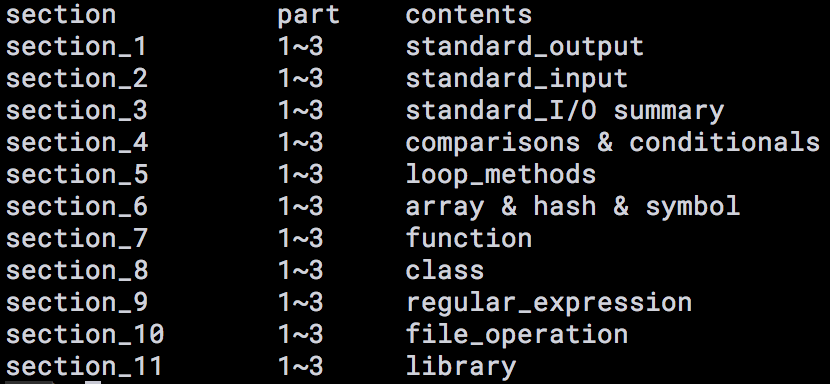
\includegraphics[width=150mm]{../../picture/seq_contents.png}
\end{center}
\caption{教材内容.\label{seq_contents}}
\end{figure}

\section{課題}\label{question}
課題は教材の各単元ごとに執筆した.使用者はこの教材で知識のアウトプットを行う.
この課題を適切に回答できれば,上記の教材から適切な知識をインプットできていると判断する.

\section{回答の評価}\label{evaluation}
使用者が作成した課題への回答が期待される振る舞いとコーディング規則に従っているかどうか評価する.
Rubyはインタプリタ言語なのでコンパイルを必要としない.
そこで,以下で解説する評価項目にシンタックスチェックは含まない.
\begin{description}
\def\labelenumi{\arabic{enumi}.}
\tightlist
\item[期待される振る舞い] 期待される振る舞いが出来ている状態とは,コードが目的を果たす動作を適切に行なっている状態のことを示す.この項目を評価する為にテストフレームワークを用いて各課題に対してのテストを用意する.このテストをクリアした場合に期待される振る舞いが果たされたとする.
\item[コーディング規約] コーディング規約とはコード作成時に設ける一定のルールの事である.コーディング規約を設ける事で可読性と保守性の向上を可能にする.この項目を評価する為に全ての課題に共通のコーディング規約を設ける.
\end{description}
上記の2つの評価の大きな流れを以下に記す.
\begin{figure}[H]
\centering
\begin{center}
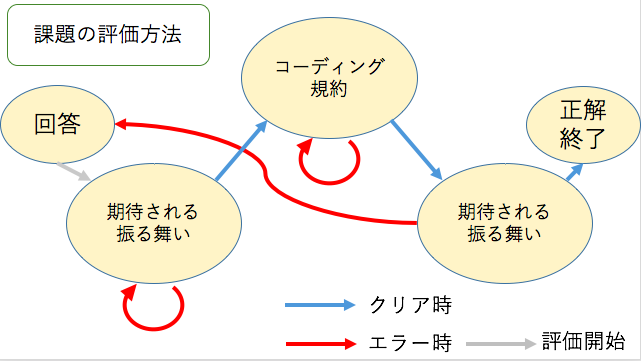
\includegraphics[width=150mm]{../../picture/seq_flow.png}
\end{center}
\caption{sequential\_checkの評価フロー.\label{seq_flow}}
\end{figure}

\section{エディタ}\label{editor}
アプリ使用者が行う課題の回答に適したエディタを決定する.
上記で本研究で開発するアプリケーションは,CUIで操作するshellを用いたアプリケーションとしているので,エディタもshell上で動作する必要がある.また,エディタにはプログラミングする上で便利な複数の機能を設定できるものを使用することで作業効率を上げることが出来る.
それを満たす一般的なエディタにはVim\cite{Vim}とEmacs\cite{Emacs}の2つが挙げられる.
西谷研究室で使用を勧めているエディタはEmacsであり,本研究では西谷研究室の早期学習を目的としているので,用いるエディタはEmacsとする.

\section{使用したgemファイル}\label{ux4f7fux7528ux3057ux305fgemux30d5ux30a1ux30a4ux30eb}
\subsection{RSpec}\label{rspec}
RSpec\cite{rspec}とはRuby用のテストフレームワークである.
本研究の教育アプリケーションが提供する学習用の課題に対して,使用者の回答が期待される振る舞いをしているかを確認する為に用いる.

\subsection{Rubocop}\label{rubocop}
Rubocop\cite{rubocop}とはコードが任意のコーディング規約に従っているかを判定するライブラリである.
本研究の教育アプリケーションが提供する学習用の課題に対して,使用者の回答がコーディング規約に従っているかを確認する為に用いる.

\subsection{Thor}\label{thor}
Thor\cite{thor}とはCLI作成支援のライブラリである.
本研究で作成する教育アプリケーションは複数の機能を内包しており,同時にCUIで実行させる必要がある.
上記を実現するためにThorを用いて開発を行う.

\section{CLI作成ツールの比較}\label{command_line}
本アプリケーションでは複数の機能を搭載するためにThorを用いて開発を行う.
しかし,他のライブラリの方が良いのではないかと疑問を持ったので,それらの比較を行う.
CLI作成ツールのライブラリとして代表的なものをいくつかが挙げると,Thor,Optparse\cite{optparse},GLI\cite{gli}である.
それらの比較結果を以下に示す.
\begin{table}[H]
\centering
\begin{center}
\caption{CLI作成ツールの比較.\label{cli_compare}}
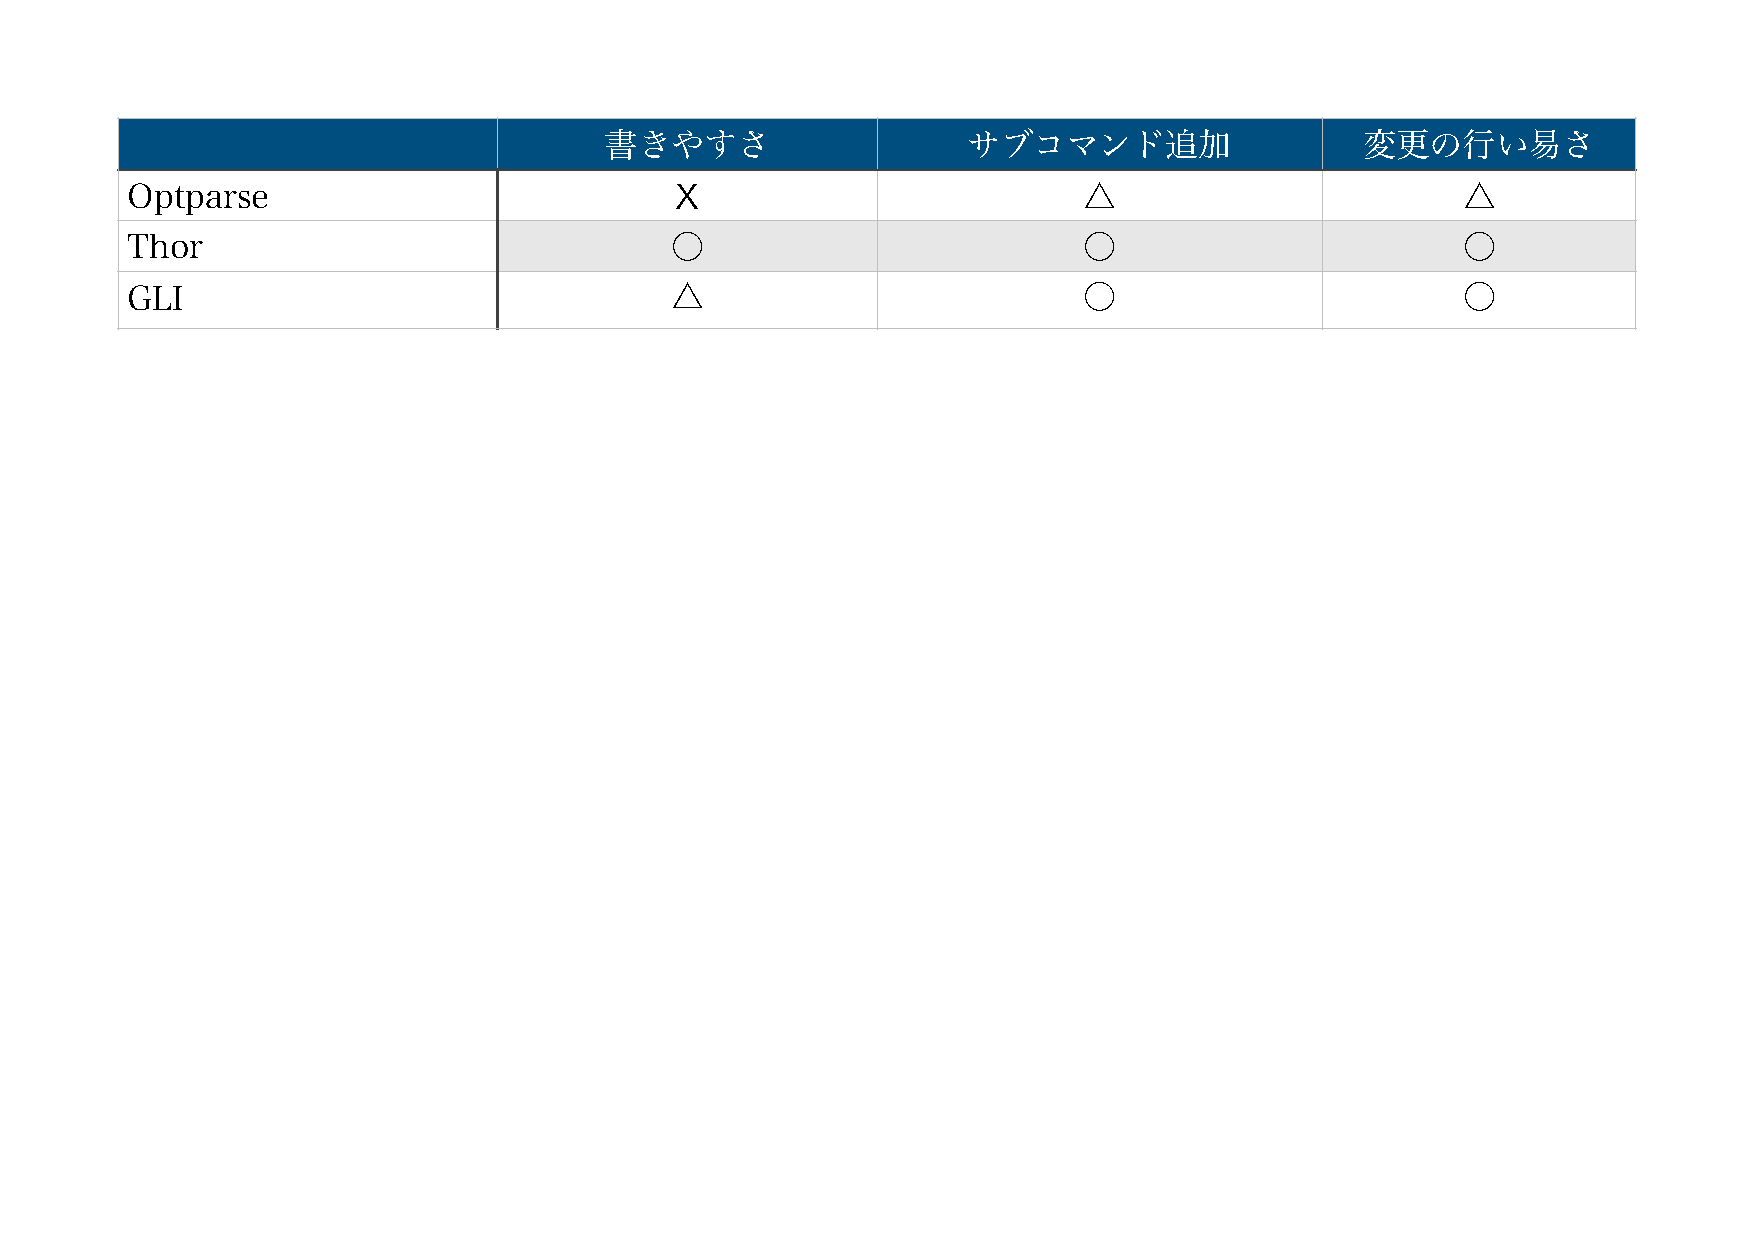
\includegraphics[width=150mm]{../../picture/cli_compare.pdf}
\end{center}
\label{fig:}
\end{table}
OptparseではOptionParserクラスを用いてCLI作成を行う.書きやすさについて他の2つと比較した際に,Optparseは独特の書き方であるのでRuby経験者であってもOptparse用に学習が必要となる.また事前に用意されたクラスを用いるのでカスタマイズが難しく,サブコマンド作成や変更作業が行いにくい.GLIとThorの比較を行う.どちらもサブコマンドの追加や変更作業は行いやすいが,コードの書きやすさについて違いがある.ThorはThorクラスの継承を行うだけで基本的なCLI作成は終了するが,GLIはRubyに似た書き方であるが1から細かく書いていかなければいけない.このそれぞれをまとめた表が上記の表である.また,インストール数には大きな差があった.
上記の表からも分かる通り,現段階で新規にCLIを作成する場合はThorを選択することが最適であると考える.
